\documentclass[tikz,convert={outfile=figure4_prisma.png}]{standalone}
\begin{document}
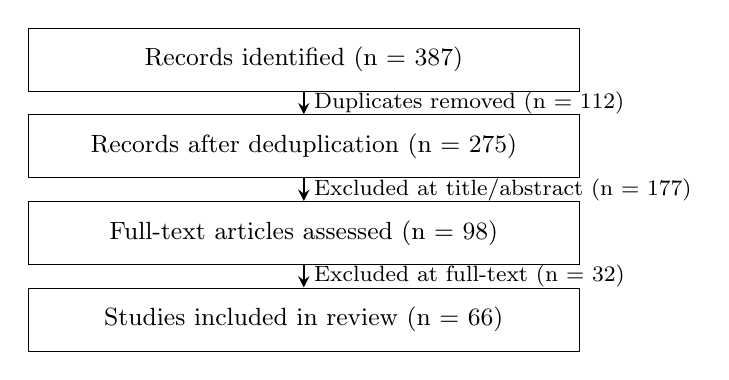
\begin{tikzpicture}[node distance=0.8cm, auto]
\tikzset{box/.style={rectangle, draw, minimum width=7cm, minimum height=0.8cm, text centered, font=\small, inner sep=4pt, fill=white}}
\tikzset{arrow/.style={->, >=stealth, thick}}

\node[box] (ident) {Records identified (n = 387)};
\node[box, below of=ident, yshift=-0.3cm] (dedup) {Records after deduplication (n = 275)};
\node[box, below of=dedup, yshift=-0.3cm] (full) {Full-text articles assessed (n = 98)};
\node[box, below of=full, yshift=-0.3cm] (incl) {Studies included in review (n = 66)};

\draw[arrow] (ident) -- node[right, font=\footnotesize] {Duplicates removed (n = 112)} (dedup);
\draw[arrow] (dedup) -- node[right, font=\footnotesize] {Excluded at title/abstract (n = 177)} (full);
\draw[arrow] (full) -- node[right, font=\footnotesize] {Excluded at full-text (n = 32)} (incl);
\end{tikzpicture}
\end{document}
